\chapter*{Création du launcher}
\addcontentsline{toc}{chapter}{Création du launcher}

\begin{center}
  \begin{figure}[ht]
    \caption{\label{mainLauncher} On fait un appel à une méthode d'une feuille depuis le classeur}
    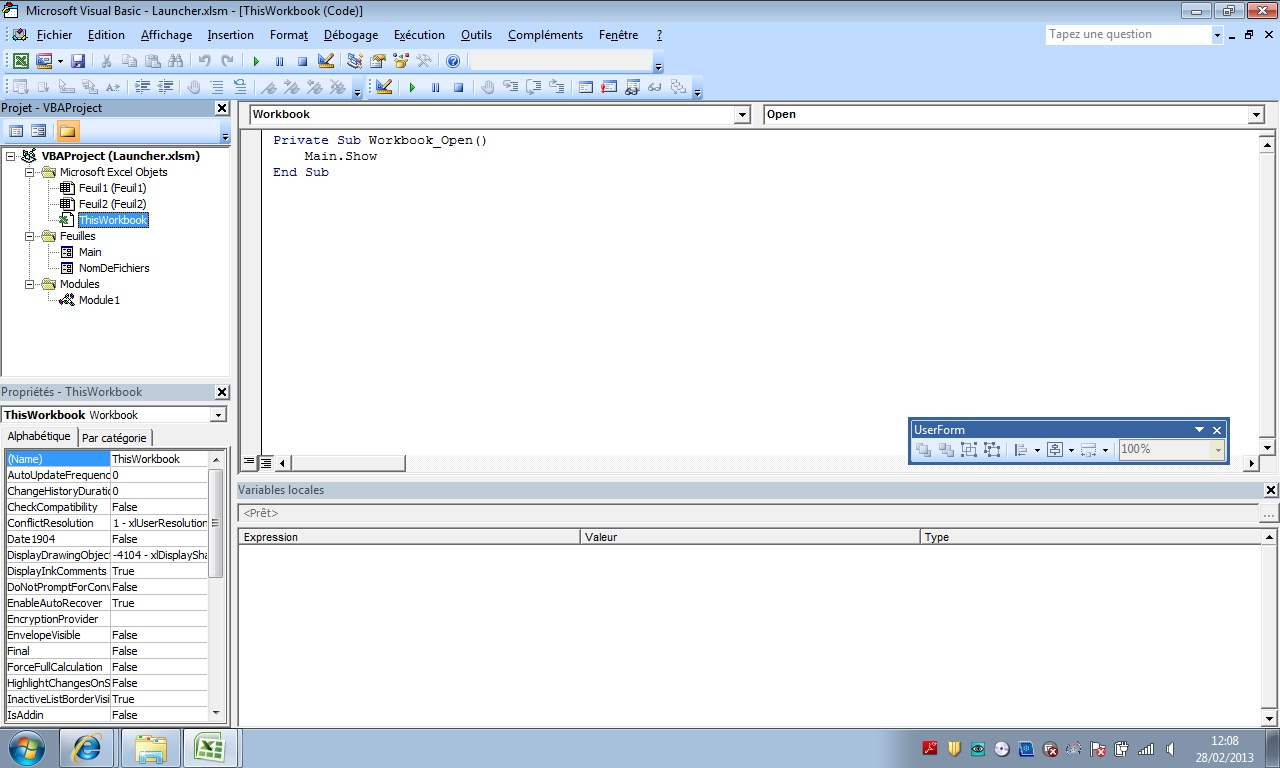
\includegraphics [width=1\textwidth]{images/aMainLauncher.jpg}
  \end{figure}
  \begin{figure}[ht]
    \caption{\label{InterfaceUserFormMain} Création d'u launcher}
    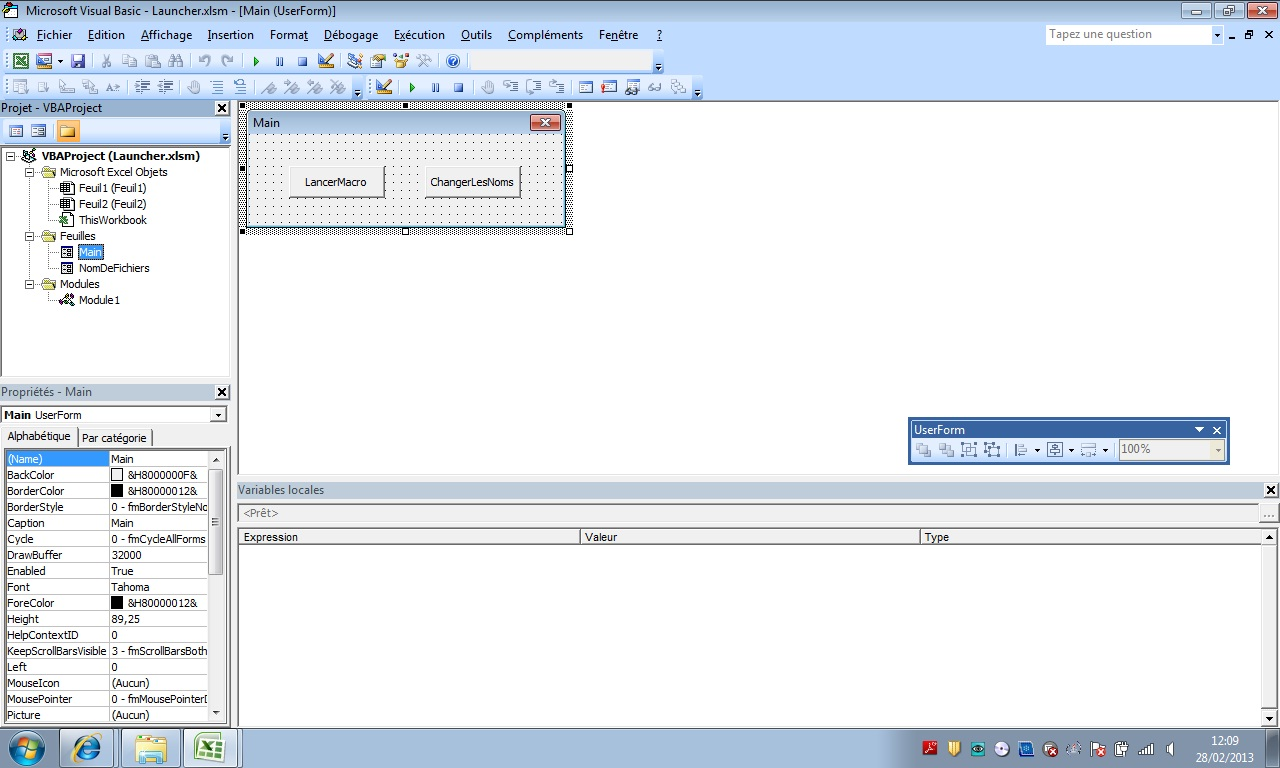
\includegraphics [width=1\textwidth]{images/InterfaceUserFormMain.jpg}
  \end{figure}
  \begin{figure}[ht]
    \caption{\label{InterfaceUserFormNoms} Création d'une boite de dialogue}
    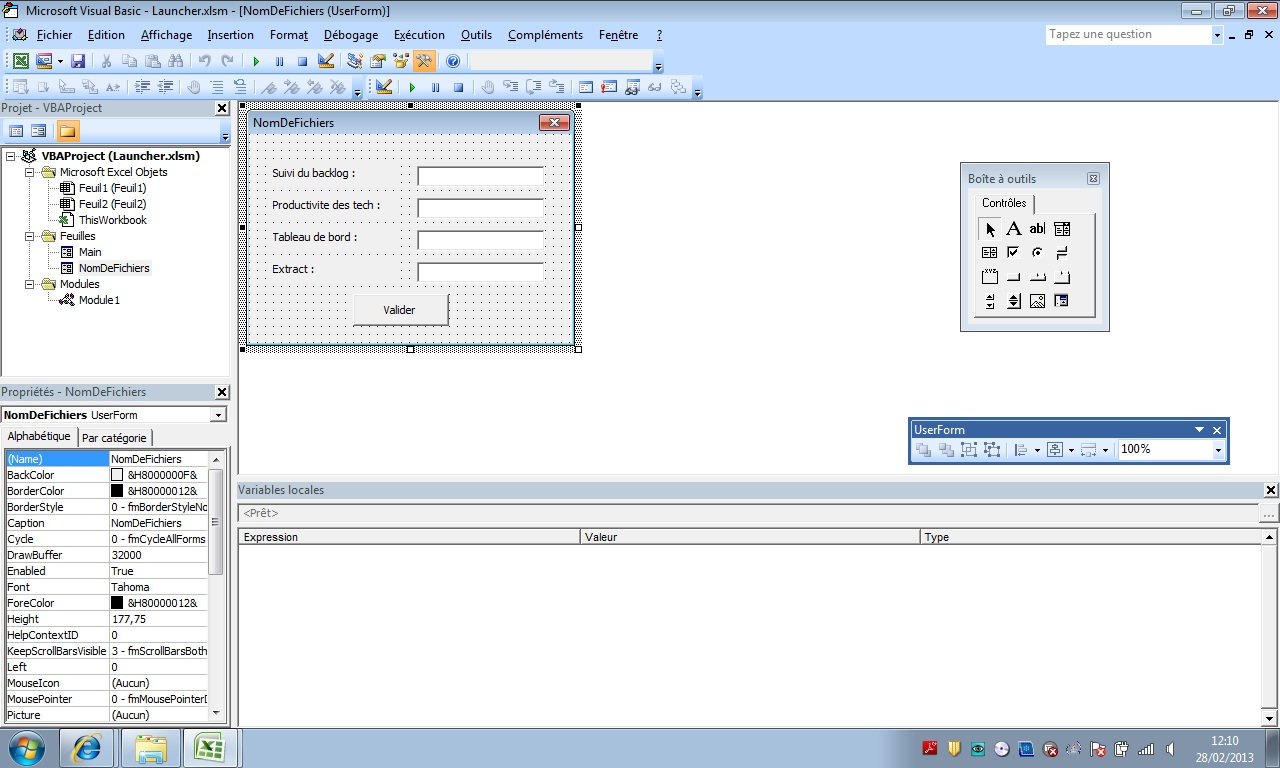
\includegraphics [width=1\textwidth]{images/InterfaceUserFormNoms.jpg}
  \end{figure}
  \begin{figure}[ht]
    \caption{\label{CodeUserFormMain} Méthodes appelés lors d'un clic sur les boutons}
    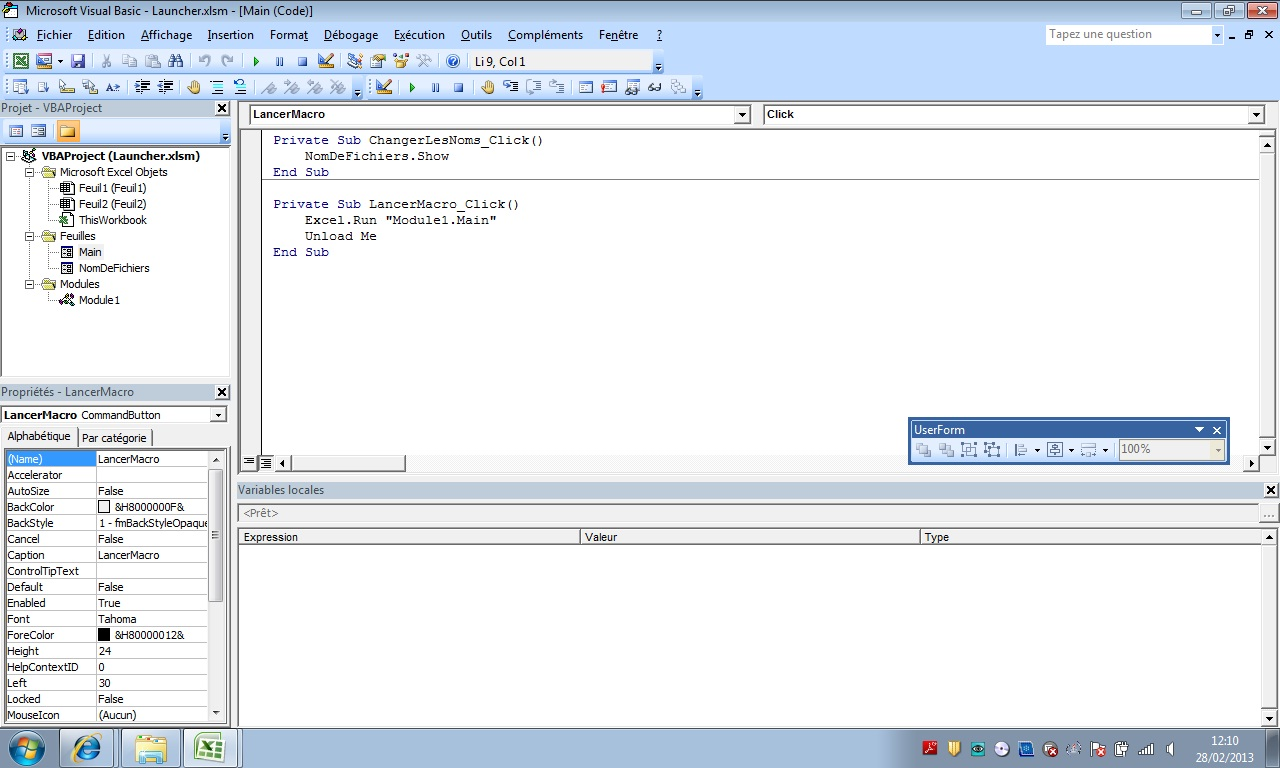
\includegraphics [width=1\textwidth]{images/code/CodeUserFormMain.jpg}
  \end{figure}
  \begin{figure}[ht]
    \caption{\label{CodeMacroLauncher} Code exécuté au clic sur le bouton "lancerMacro"}
    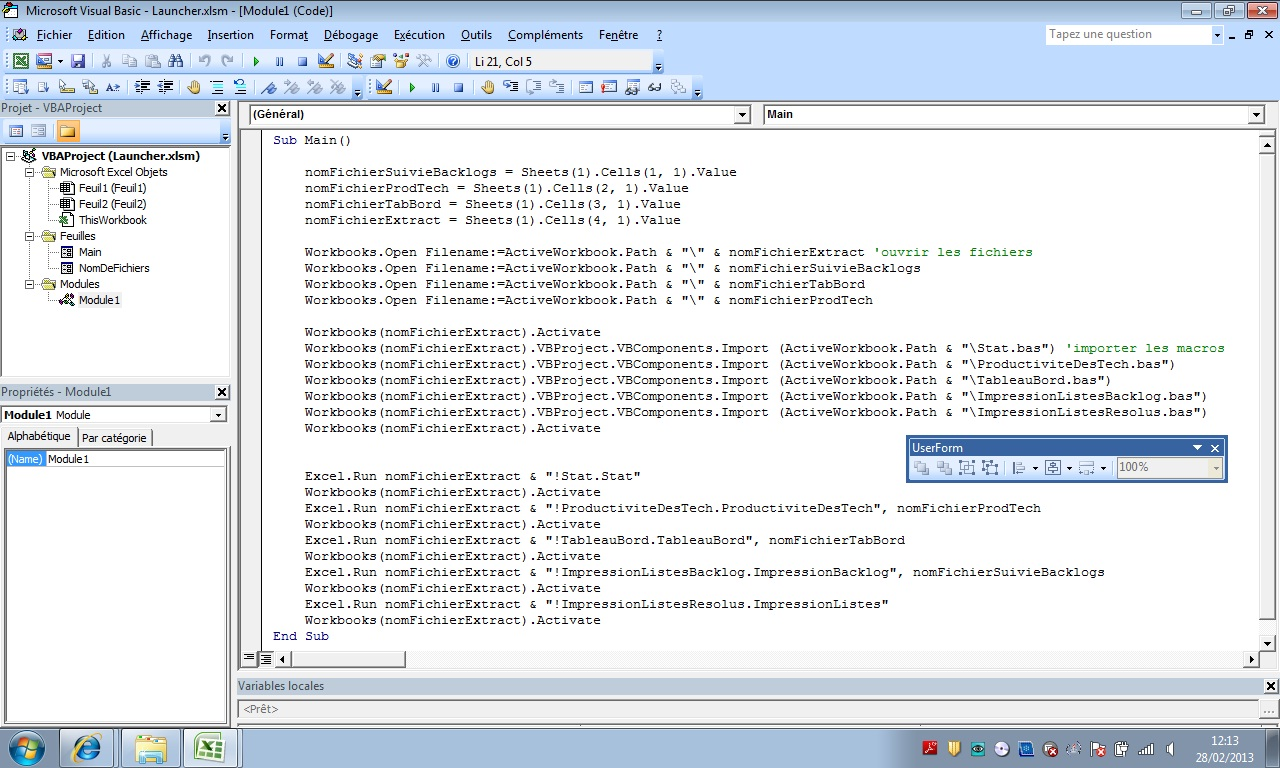
\includegraphics [width=1\textwidth]{images/code/CodeMacroLauncher.jpg}
  \end{figure}
  \begin{figure}[ht]
    \caption{\label{CodeUserFormNoms} Code exécuté au clic sur le bouton "changerLesNoms"}
    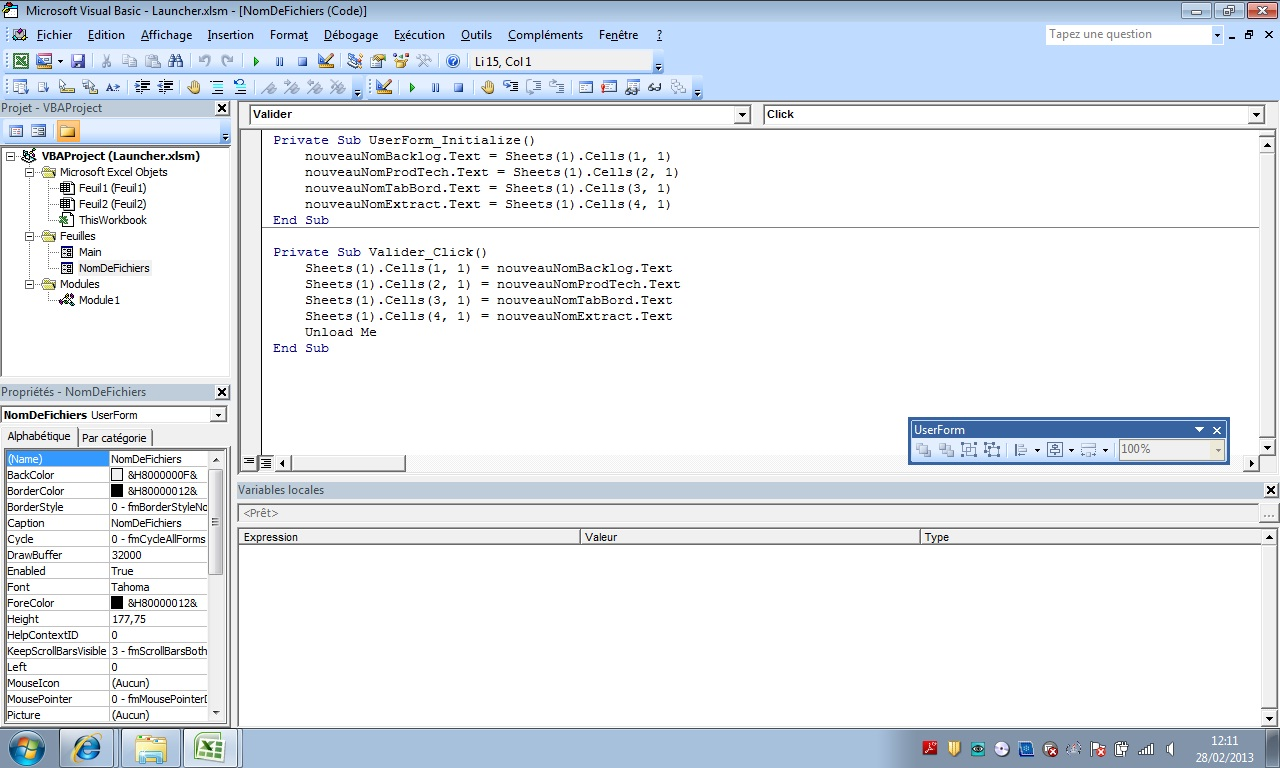
\includegraphics [width=1\textwidth]{images/code/CodeUserFormNoms.jpg}
  \end{figure}
  \begin{figure}[ht]
    \caption{\label{CodeMacroProdTechAnnexe} Code de la macro "productiviteDesTechs"}
    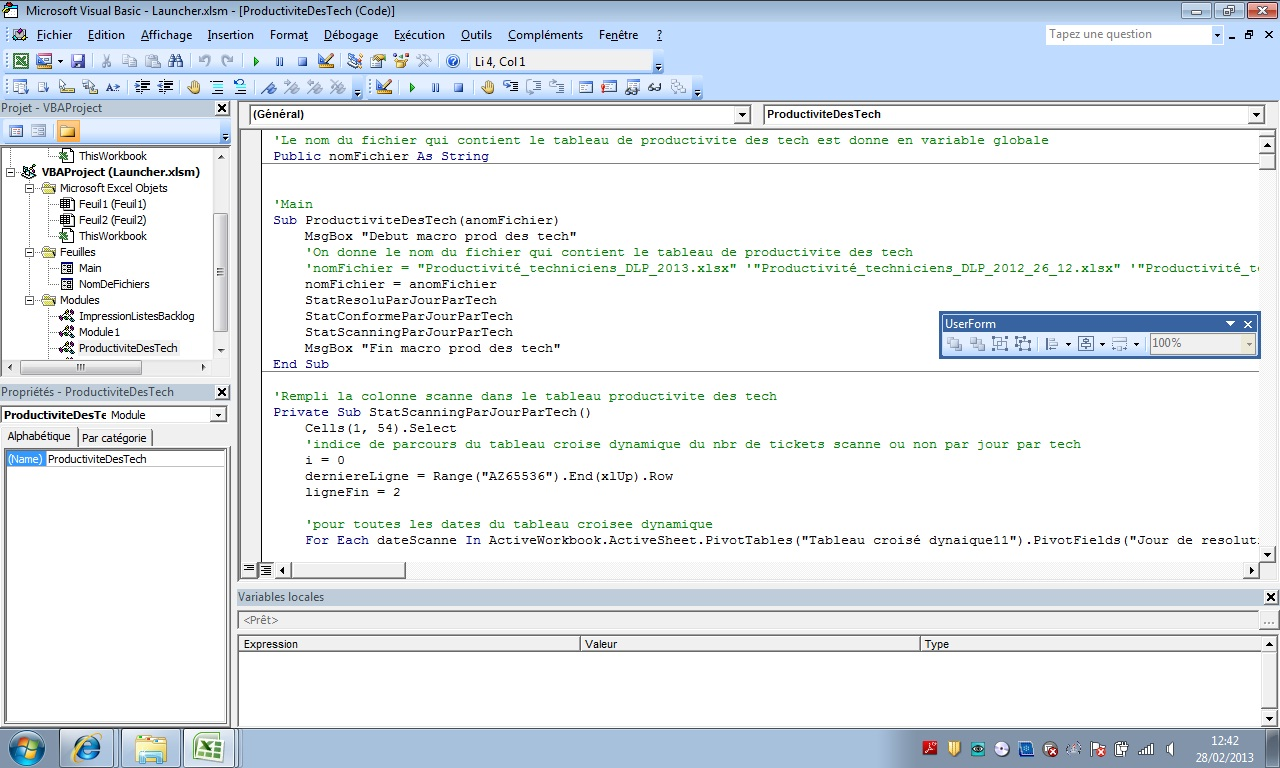
\includegraphics [width=1\textwidth]{images/code/CodeMacroProdTechAnnexe.jpg}
  \end{figure}
\end{center}

\cleardoublepage
\chapter*{Documention}
\addcontentsline{toc}{chapter}{Documention}


\begin{center}
\textbf{HowTo Launcher}
\end{center}
\lstinputlisting{doc/HowTo.txt}

\begin{center}
\textbf{Doc Launcher}
\end{center}
\lstinputlisting{doc/readmeLauncher.txt}

\begin{center}
\textbf{Doc généralee}
\end{center}
\lstinputlisting[breaklines]{doc/readmeMain.txt}

\begin{center}
\textbf{Doc macro contrôle}
\end{center}
\lstinputlisting[breaklines]{doc/readmeStats.txt}

\cleardoublepage
\chapter*{Matériel dépanné et locaux}
\addcontentsline{toc}{chapter}{Matériel dépanné}

\begin{center}
  \begin{figure}[ht]
    \caption{\label{tpe} Quelques appareils réparé (scannette(g), terminal de paiement électronique, imprimante à tickets de caisse(d)"}
    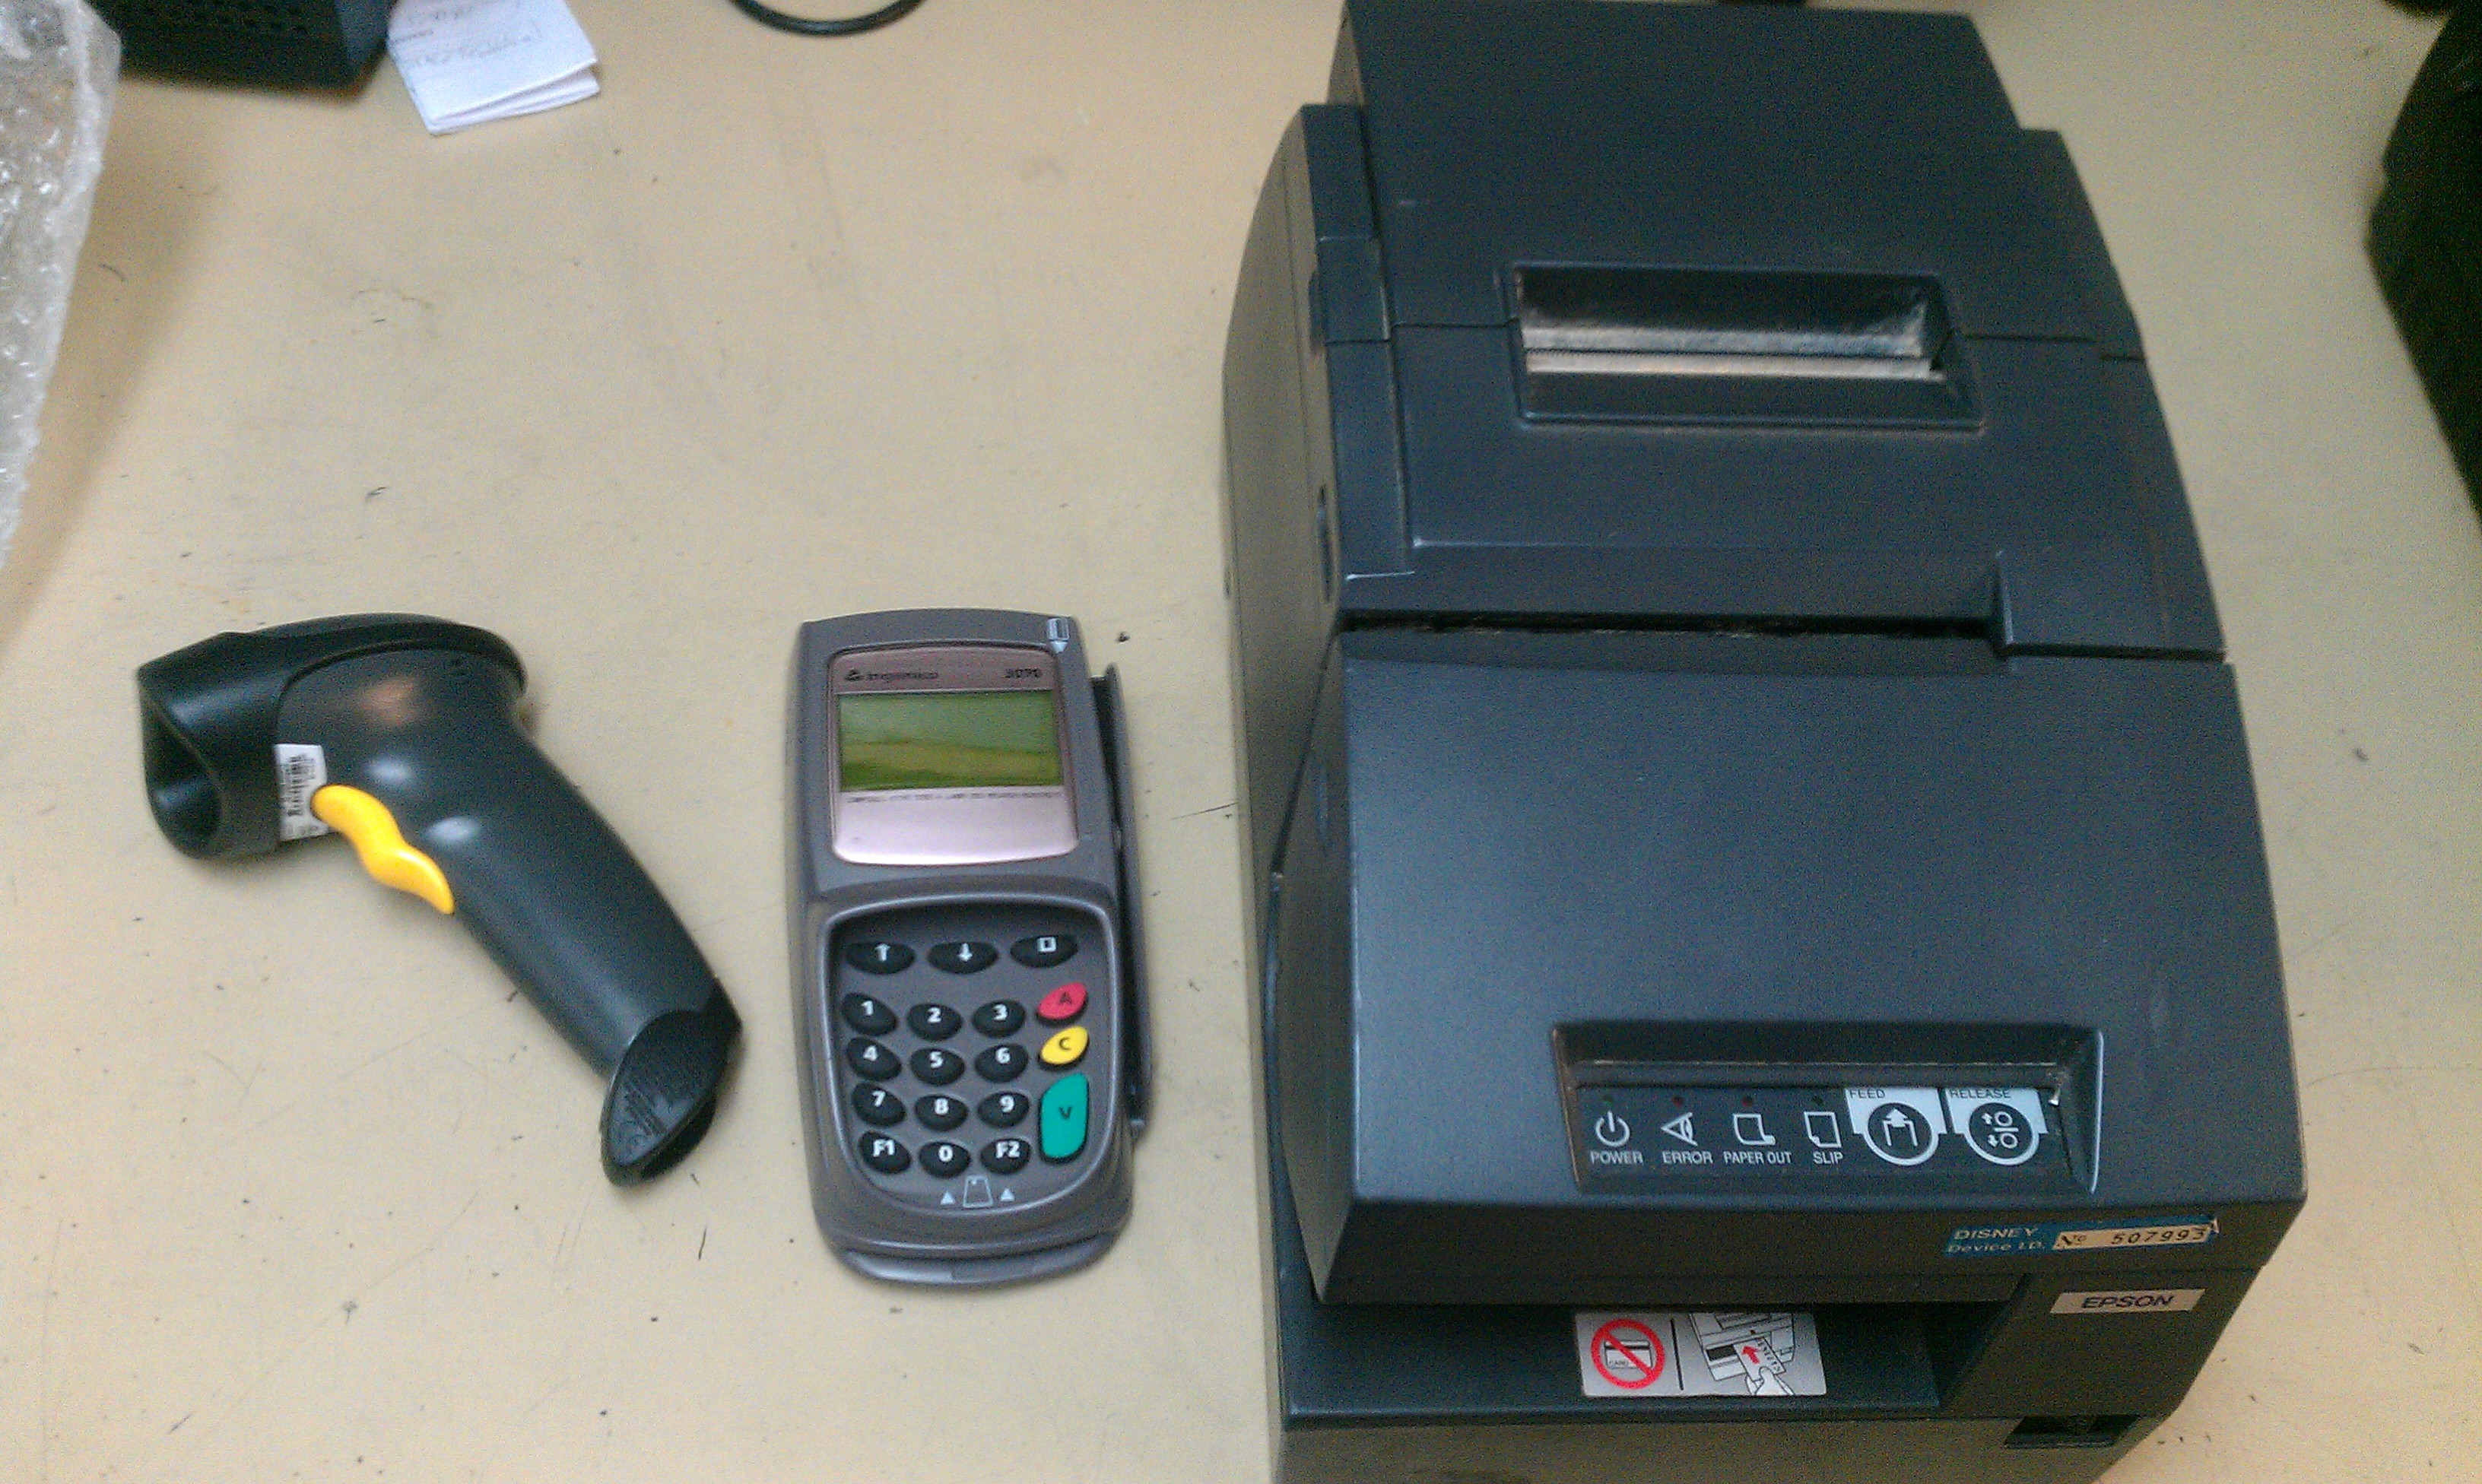
\includegraphics [width=1\textwidth]{images/tpe.jpg}
  \end{figure}
  \begin{figure}[ht]
    \caption{Le stock}
    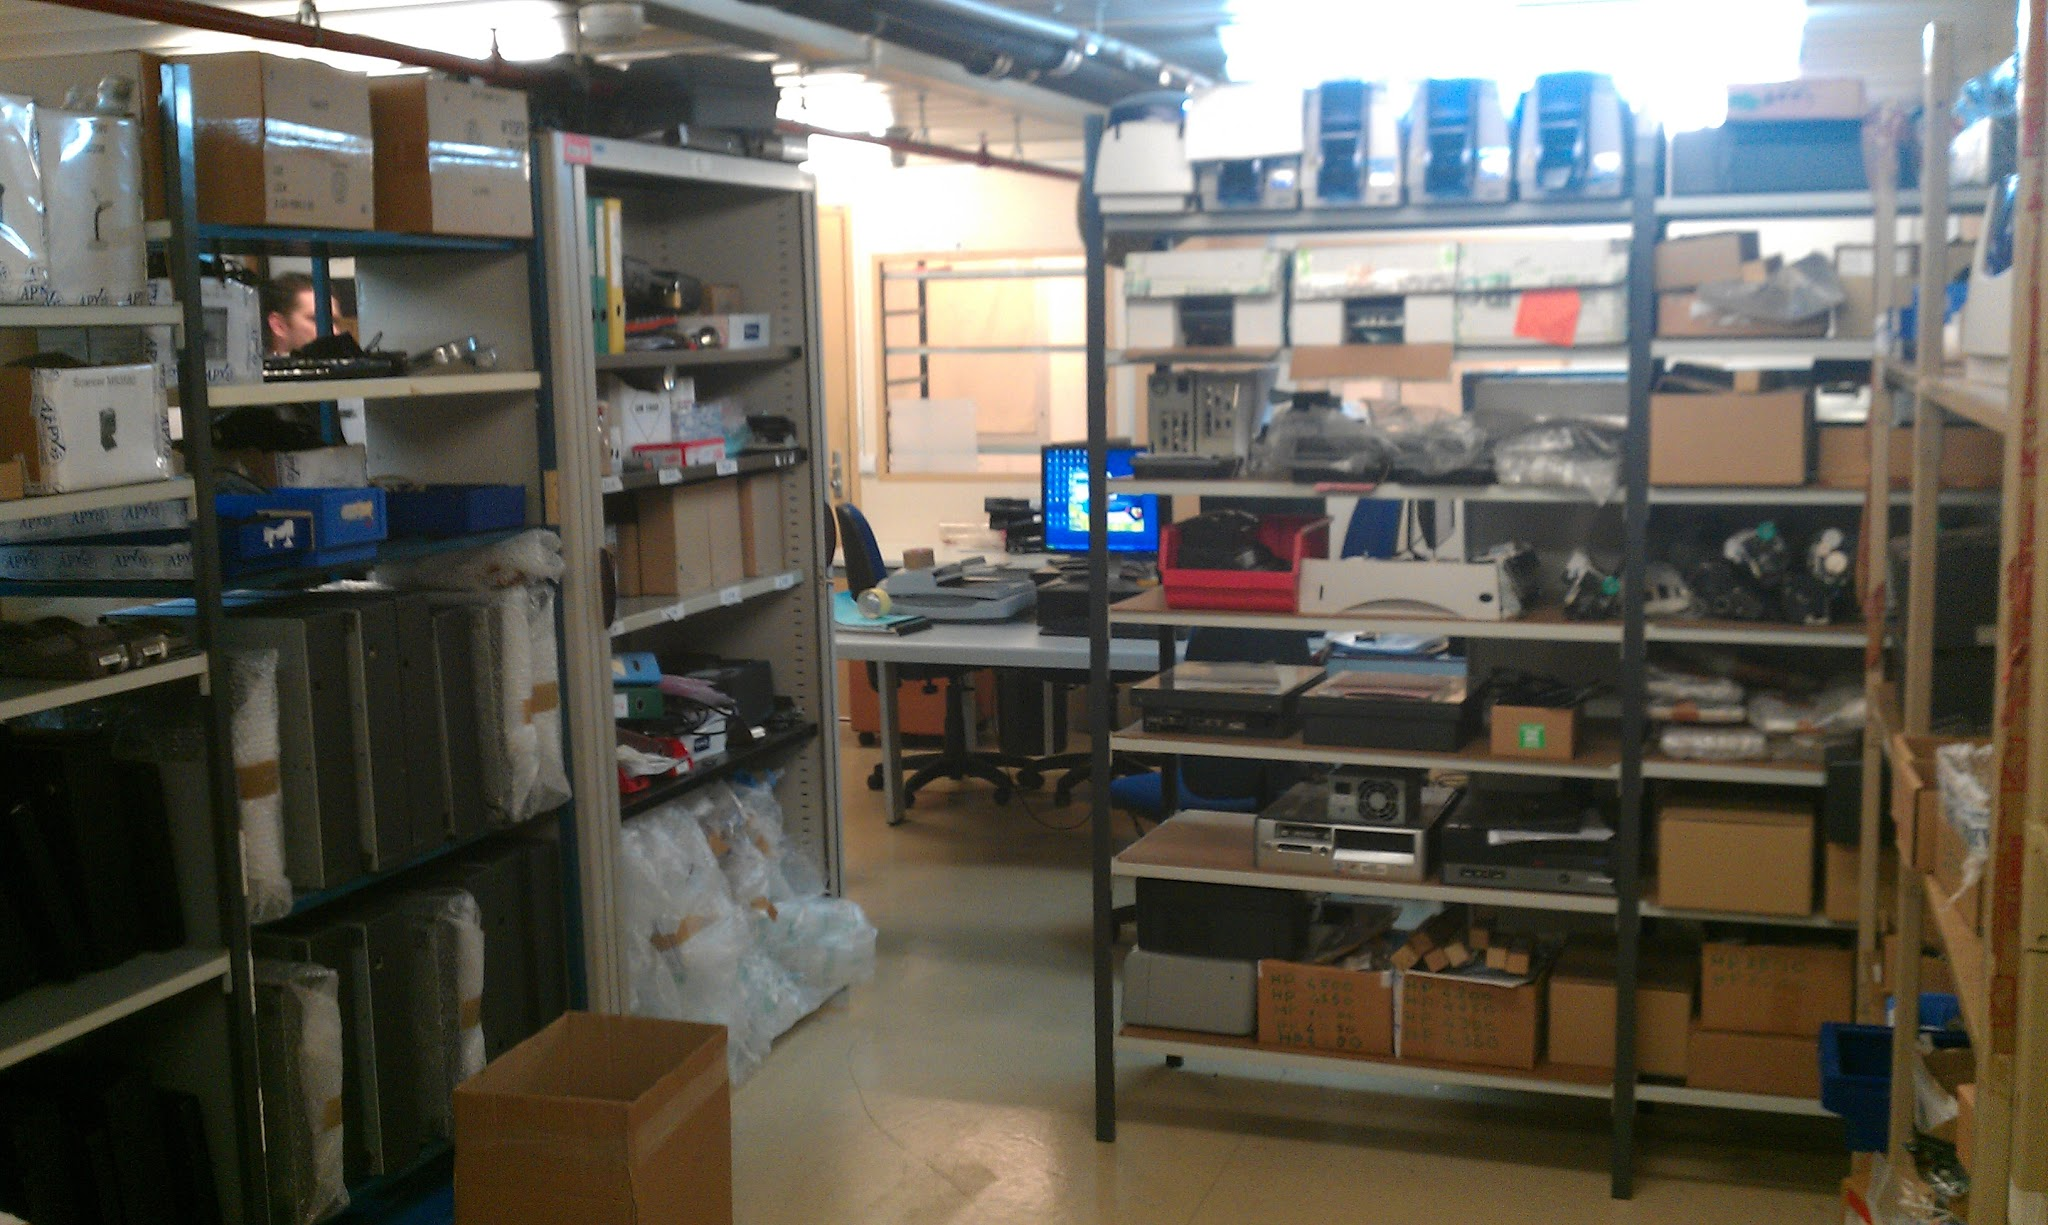
\includegraphics [width=1\textwidth]{images/locaux/IMAG0392.jpg}
  \end{figure}
  \begin{figure}[ht]
    \caption{Le stock}
    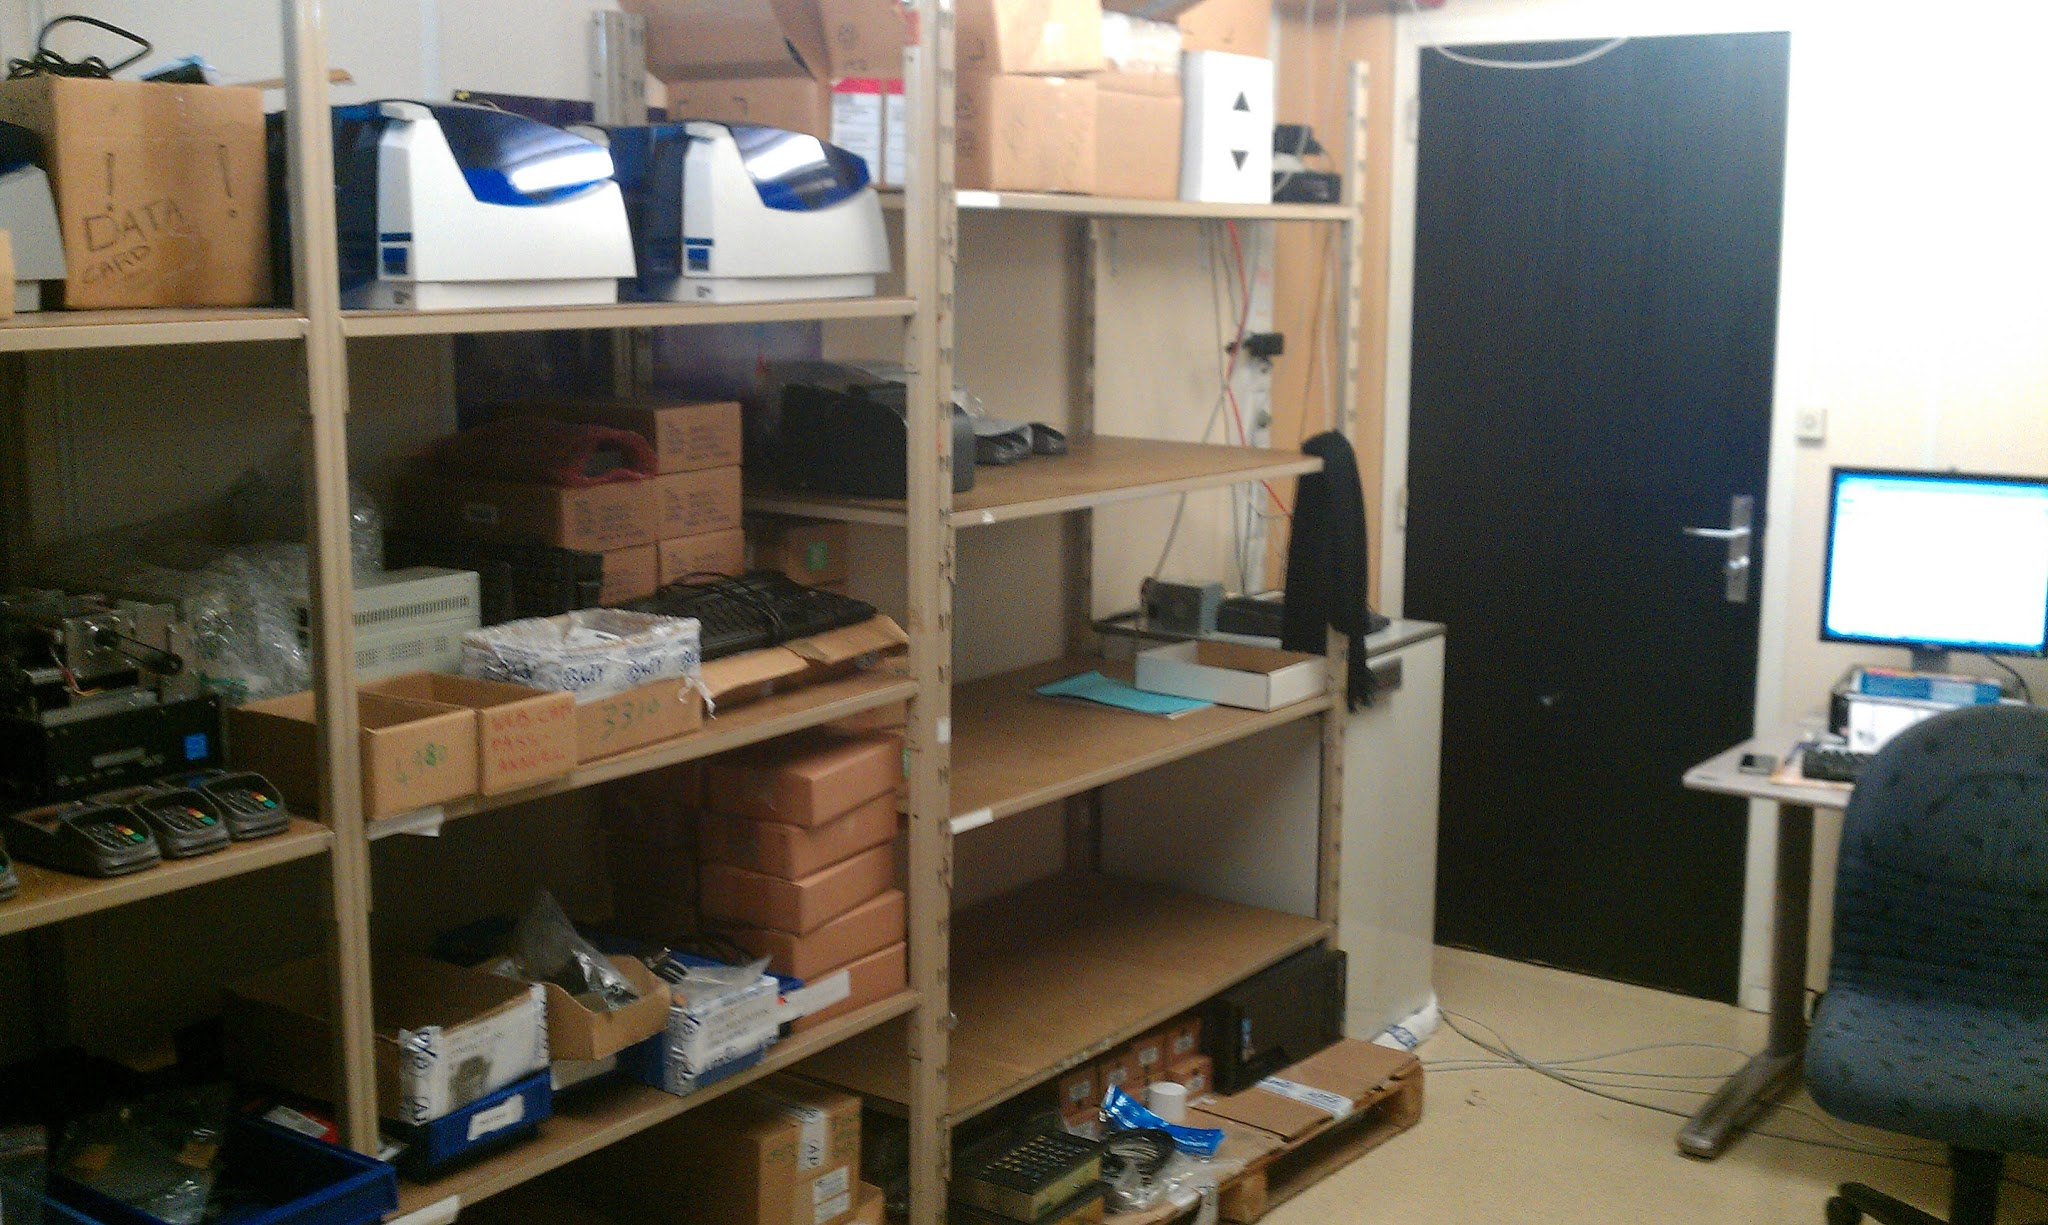
\includegraphics [width=1\textwidth]{images/locaux/IMAG0395.jpg}
  \end{figure}
  \begin{figure}[ht]
    \caption{Les bureaux}
    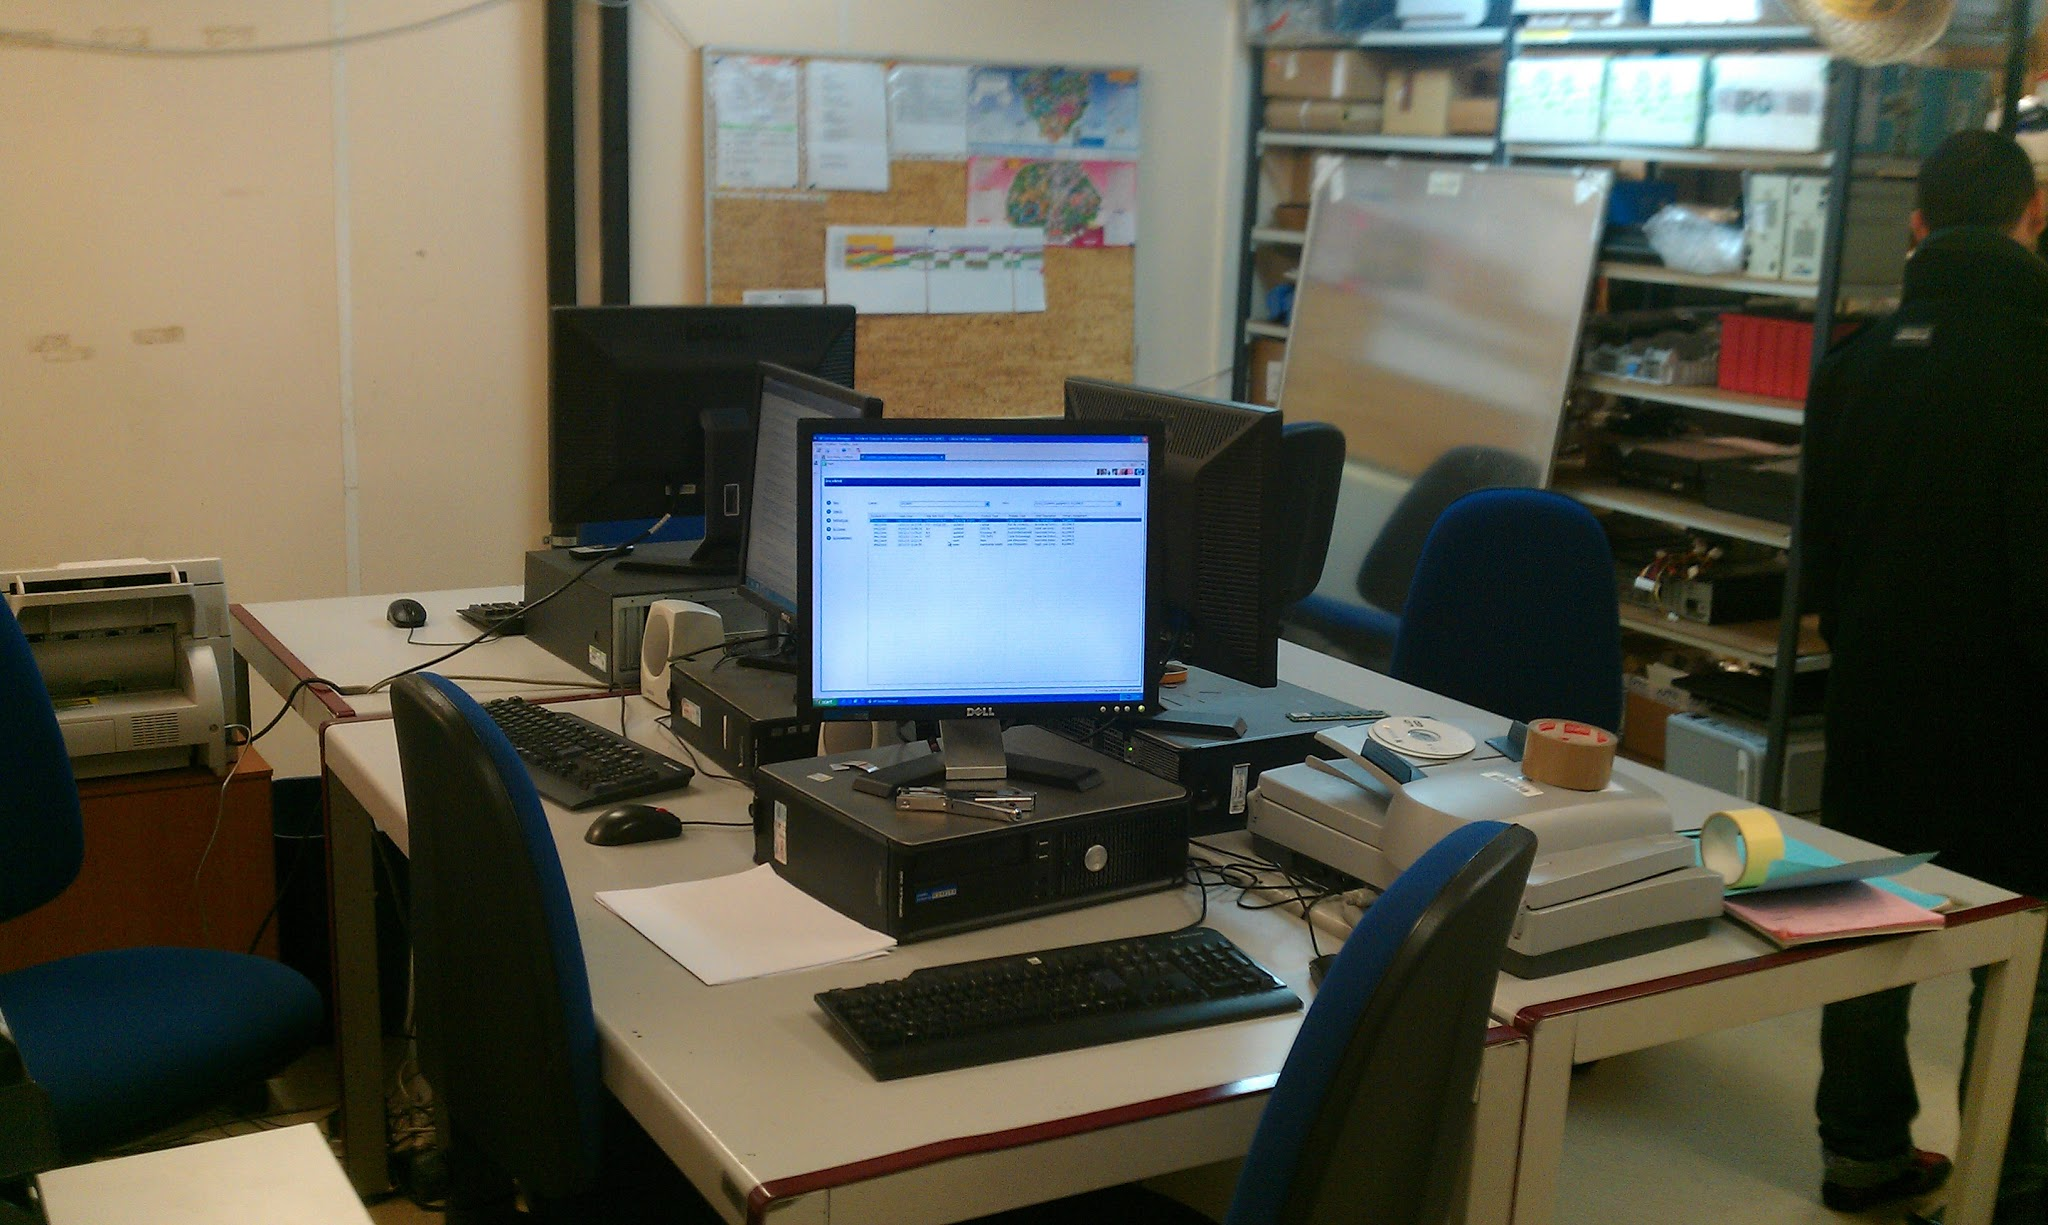
\includegraphics [width=1\textwidth]{images/locaux/IMAG0393.jpg}
  \end{figure}
  \begin{figure}[ht]
    \caption{Les bureaux}
    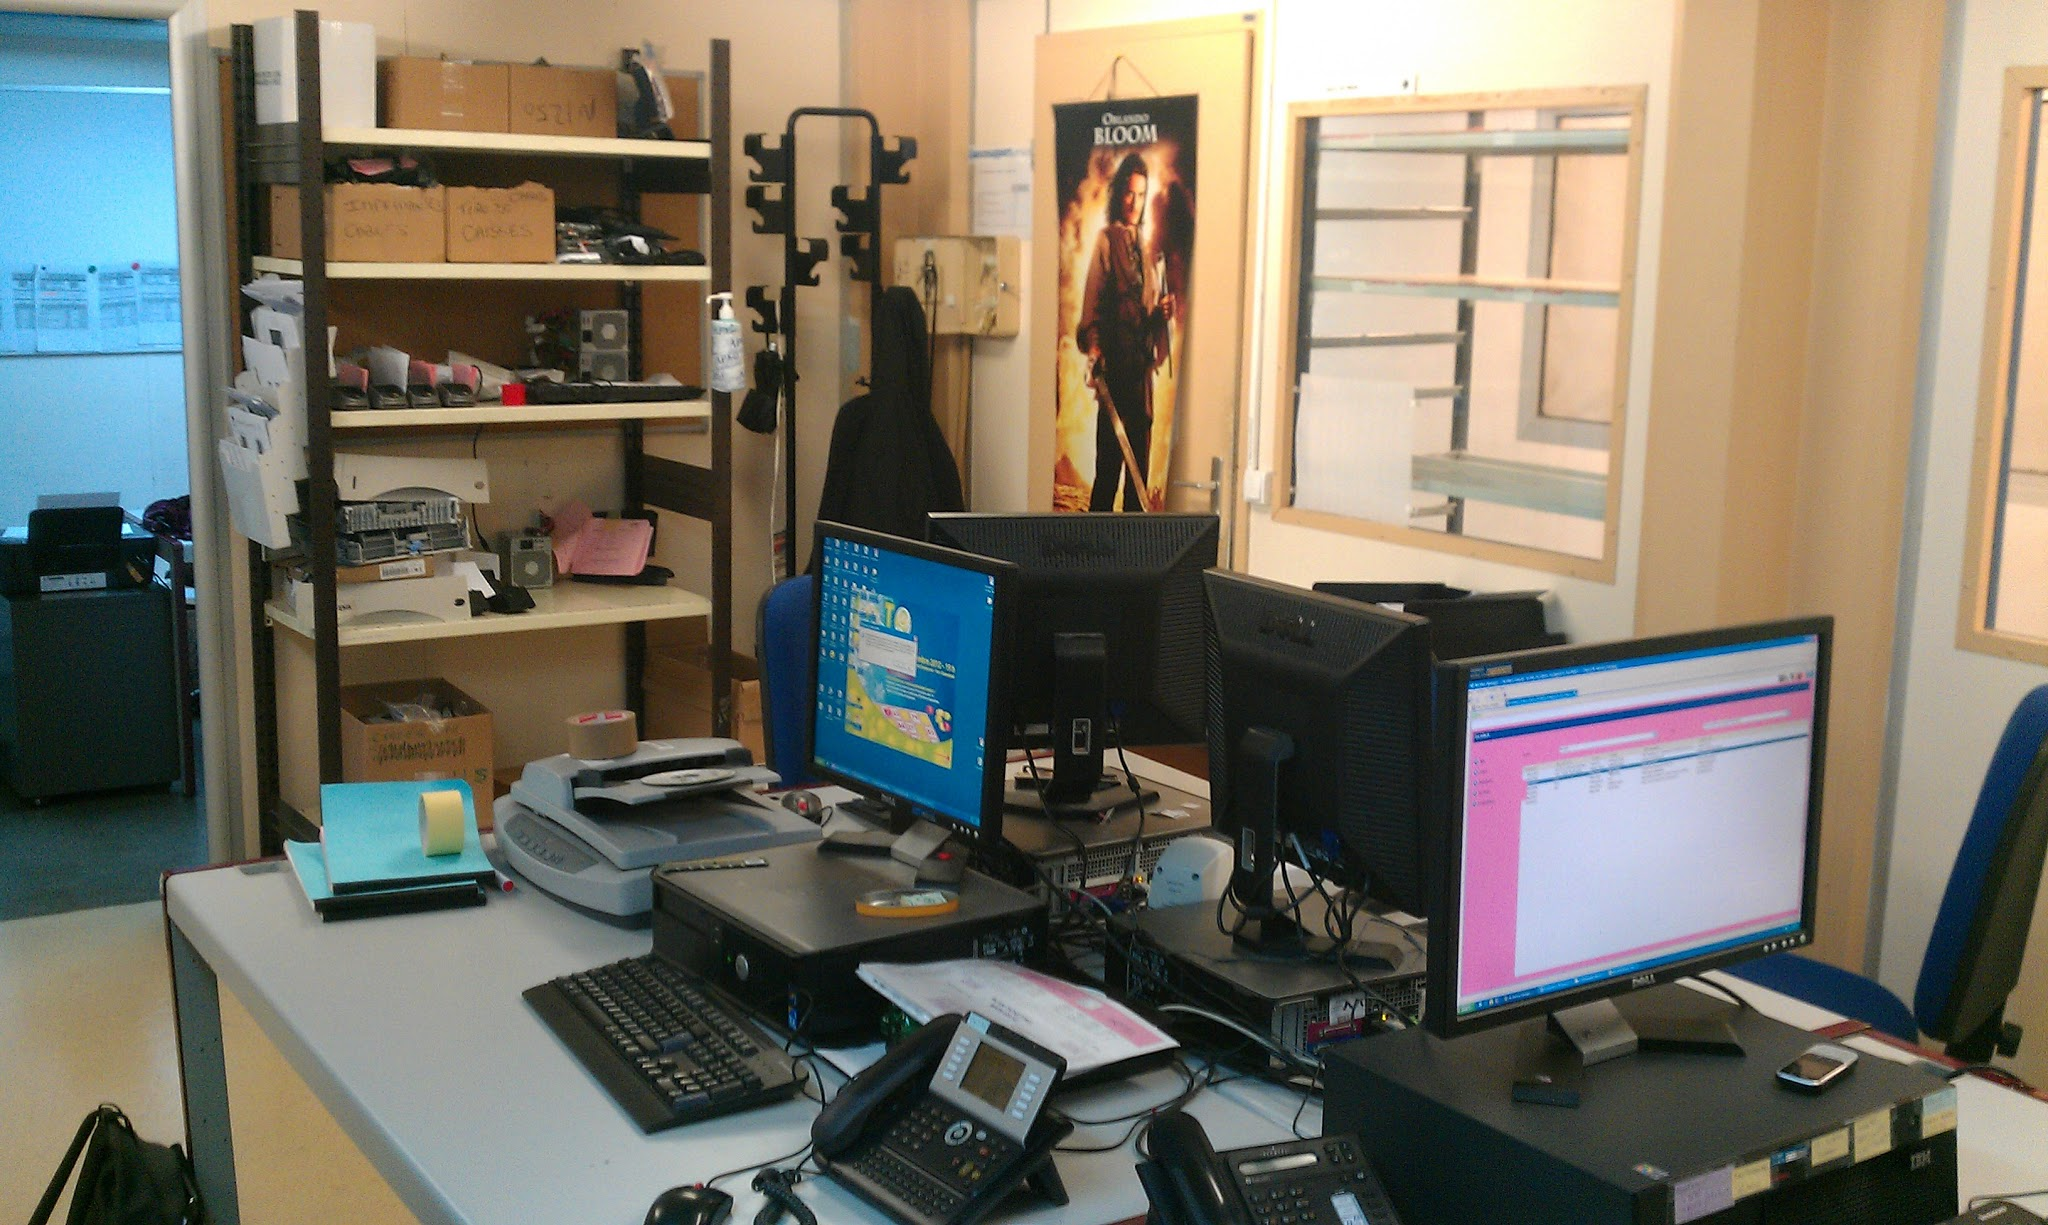
\includegraphics [width=1\textwidth]{images/locaux/IMAG0398.jpg}
  \end{figure}
  \begin{figure}[ht]
    \caption{Le bureau de la chef}
    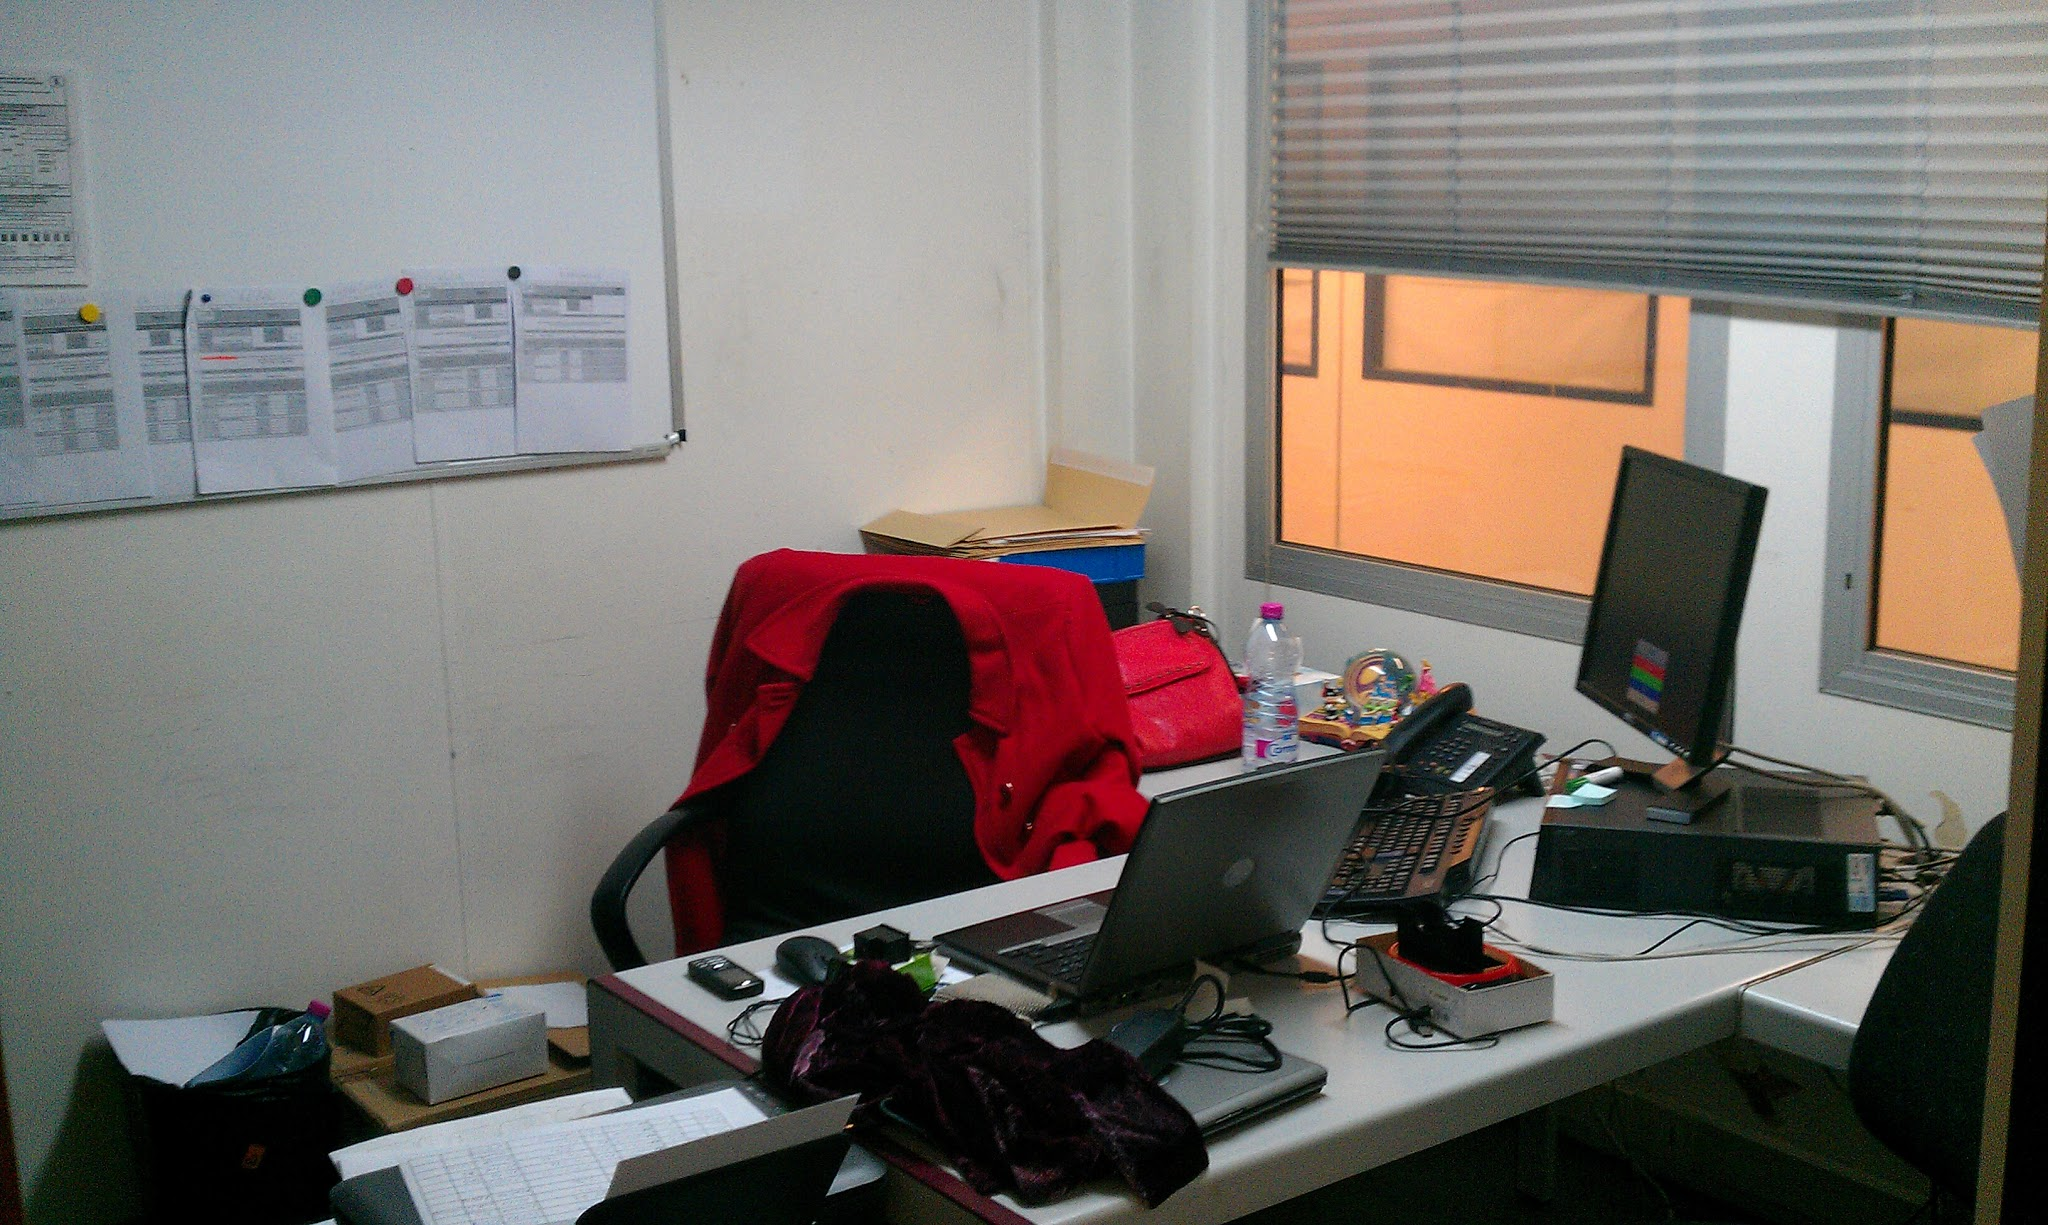
\includegraphics [width=1\textwidth]{images/locaux/IMAG0399.jpg}
  \end{figure}
  \begin{figure}[ht]
    \caption{L'atelier}
    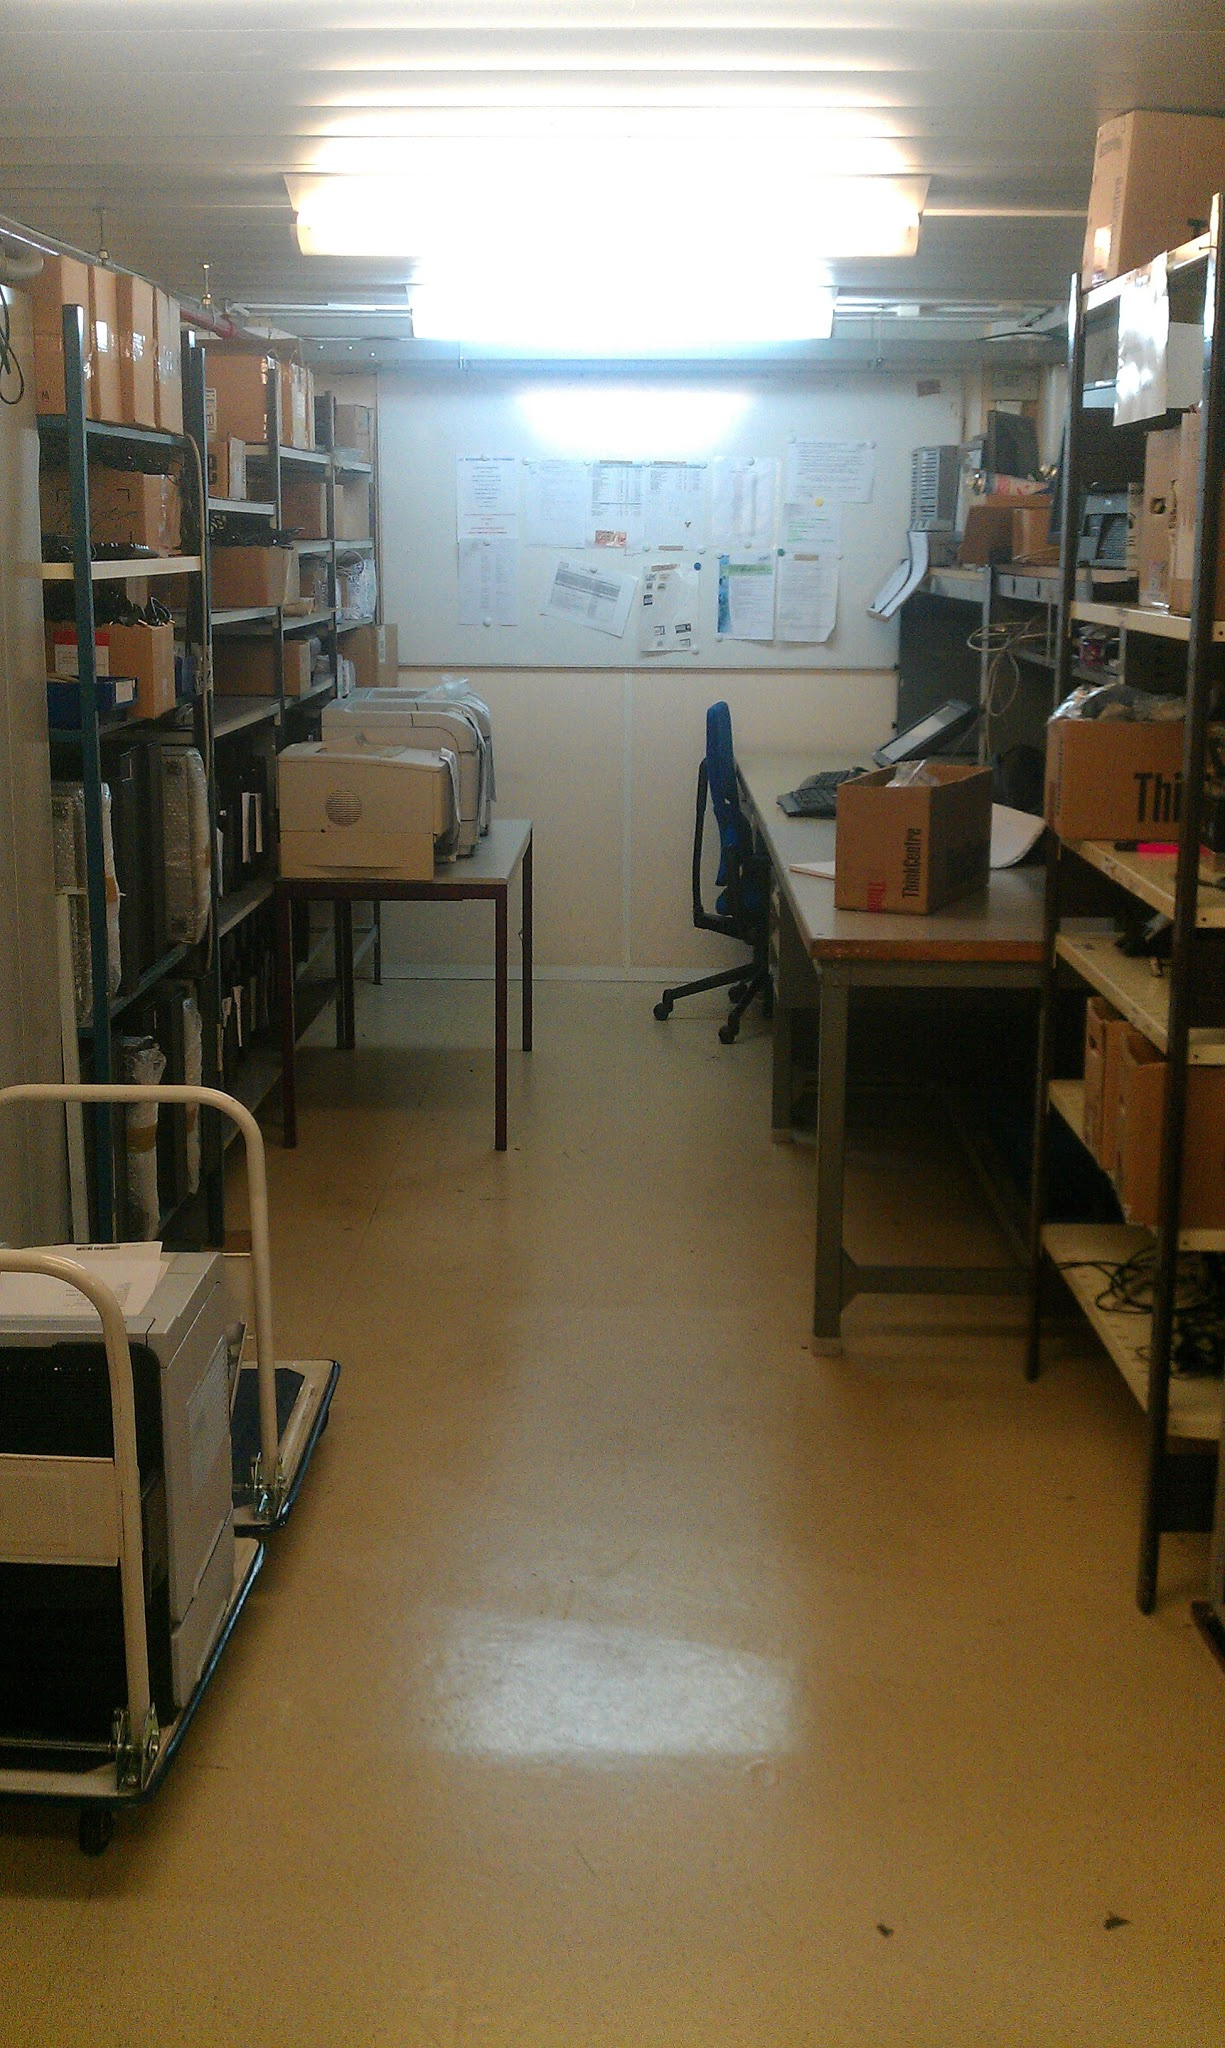
\includegraphics [width=1\textwidth, height=0.8\textheight]{images/locaux/IMAG0400.jpg}
  \end{figure}
\end{center}

\cleardoublepage
\chapter*{SM7}
\addcontentsline{toc}{chapter}{SM7}

\begin{center}
  \begin{figure}[ht]
    \caption{SM7}
    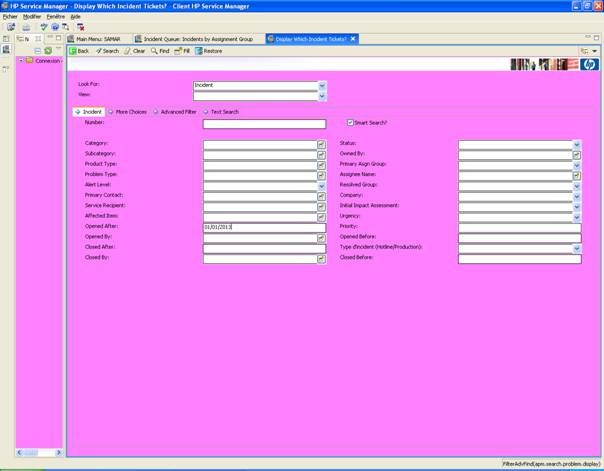
\includegraphics [width=1\textwidth]{images/sm7annexe/image001.jpg}
  \end{figure}
  \begin{figure}[ht]
    \caption{SM7}
    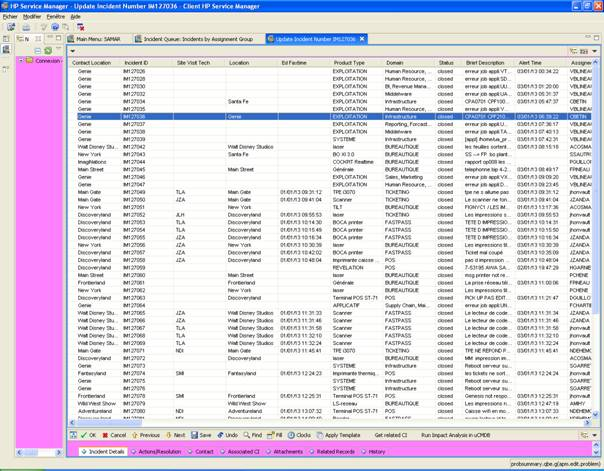
\includegraphics [width=1\textwidth]{images/sm7annexe/image002.jpg}
  \end{figure}
\end{center}

\cleardoublepage
\chapter*{Alloy}
\addcontentsline{toc}{chapter}{Alloy}

\begin{center}
\textbf{Modèle Alloy}
\end{center}
\lstinputlisting[breaklines]{images/alloy/essaiEDTV2.als}

